\subsubsection{Generalized Auto-Regressive Conditional Heteroskedasticity}
Теперь рассматриваем следующее соображение: глядя на график доходностей Apple за 2021 год (для цен открытия), видно, что в какие-то моменты волатильность больше, а в какие-то меньше. 
\begin{figure}[H]
	\centering
	\begin{tikzpicture}
		\begin{axis}[
			grid = both,
			legend pos = north west,
			minor tick num = 1,
			major grid style = {lightgray},
			minor grid style = {lightgray!25},
			xlabel = {2021 год},
			width = 1.025 \textwidth,
			height = 0.5 \textwidth,
			xmin=-5, xmax=260,
			% ymin=115, ymax=185,
			xtick={0, 40, 80, 120, 160, 200, 240},
			xticklabels={03/01, 02/03, 28/04, 24/06, 20/08, 18/10, 14/12},
			line width=0.3mm
			]
			\addplot table [
			x=x, 
			y=Open_pct, 
			col sep=comma,
			mark={},
			] {./source/source_csv/Illustration data/apple_data_test_pct.csv};
			\legend{AAPL 2021}
		\end{axis}
	\end{tikzpicture}
	\caption{Доходности цен открытия акций Apple (AAPL) 2021 (\%)}
	\label{fig::apple_returns_2021}
\end{figure}
Данное явление носит название "кластеризация волатильности". Было бы неплохо научиться ее предсказывать, для чего и была разработана модель ARCH \cite{robert1982arch} и как ее обобщение - модель GARCH \cite{bollerslev1986garch}. Для большей простоты в понимании рассматриваем первоначально ARCH, а затем - GARCH.
\begin{enumerate}
	\item Пусть есть некоторая модель (неважно какая конкретно - Constant, ARIMA, ADL, DL, однако требуем, чтобы исследуемый процесс был стационарен). Тогда, представляем исследуемую модель в формальном виде:
	\begin{equation}
		\begin{split}
			y_t & = \mu_t + u_t\\
			\mu_t & \Rightarrow \text{моделирование среднего значения}\\
			u_t & = \sigma_t \varepsilon_t \\
			\sigma_t^2 & = \omega + \sum_{j = 1}^p \alpha_j u_{t - j}^2 \Rightarrow \text{моделирование условной дисперсии}
		\end{split}
	\end{equation}
	Где $\omega$ - константа, $\mu_t$ - предсказание среднего значения некоторой моделью, $u_t$ - некоторая величина, зависящая от своих предыдущих значений, $\sigma_t$ и $\varepsilon_{t}$, где $\sigma_t$ - показатель характеризующий волатильность, а $\varepsilon_t \sim N(0, 1)$ то есть - случайные шоки. Тогда, вычисляя условную дисперсию $u_t$ и математическое ожидание соответственно, получаем:
	\begin{equation}
		\begin{split}
			\V(u_t) & = \sigma^2_t  = \V(u_t \vert u_{t - 1}, \ldots, u_{t - p}) = \omega + \sum_{j = 1}^p \alpha_j u_{t - j}^2\\
			\E(\sigma^2_t) & = \sigma^2 = \E\left(\omega + \sum_{j = 1}^p \alpha_j u_{t - j}^2\right) = \omega + \sum_{j = 1}^p \alpha_j \sigma^2\\
			\sigma^2 & = \frac{\omega}{1 - \sum_{j = 1}^p \alpha_j}
		\end{split}
	\end{equation}
	При этом, в силу неотрицательности дисперсии, необходимо учитывать, что $\alpha_j > 0: j = \overline{1,p}$. Также $\E(\sigma^2_t) = \E(u^2_t) - \E(u_t)\E(u_t) = \sigma^2$. Более того, при этом $\E(u_t) = \E(\varepsilon_t) \cdot \sqrt{\cdot}$, но для большей ясности расписываем $\cov(u_{t}, u_{t - 1} \vert u_{t - 2}, \ldots, u_{t - p}) = \cov(\varepsilon_{t} \cdot \sqrt{\omega + \alpha_1 u_{t - 1}^2 + \ldots}, \varepsilon_{t - 1} \cdot \sqrt{\cdot}) = \sqrt{\cdot} \cdot \E(\varepsilon_{t}\varepsilon_{t - 1} \cdot \sqrt{\omega + \alpha_1 u_{t - 1} + \ldots}) - \E(\sqrt{\cdot} \cdot \varepsilon_{t}) \E(\varepsilon_{t - 1}) = \ldots \cdot \E(\varepsilon_{t}) \cdot \E(\varepsilon_{t - 1}) = 0$. Таким образом показано, что $\cov(u_{t}, u_{t - 1}) = 0$, однако появляется закономерный вопрос. \textbf{Q}: Каким образом данная модель поддается оценке? \textbf{A}: Посредством Метода Максимального Правдоподобия.
	
	\item Теперь рассматриваем обобщение ARCH на более высокий уровень. Предполагается наличие зависимости между $\sigma^2_t$ и $u^2_{t - p}$, а также предыдущими значениями $\sigma^2_{t - q}$, что в формальном смысле приобретает вид:
	\begin{equation}
		\sigma^2_t = \omega + \sum_{j = 1}^p \alpha_j u_{t - j}^2 + \sum_{i = 1}^q \phi_i \sigma^2_{t - i}
	\end{equation}
\end{enumerate}
Таким образом, получаем модель, способную предсказывать волатильность доходности, но не саму доходность как таковую. Данное замечание крайне важно в условии моделей условной гетероскедастичности, так как прогнозированием именно показателя доходности выступает выбранная для $\mu_t$ модель. Существуют и иные дополнения модели: FIGARCH (\myref{link::figarch}), а также TGARCH (Threshold GARCH) и EGARCH (Exponential GARCH) и так далее. Более подробно о них в \cite{verbik_econometrics_garchs}. Вывод является то, что данная модель предоставляет возможность предсказывать не саму зависимую переменную ($y_t$), а ее волатильность ($u_t$). Наиболее часто применяется GARCH$(1, 1)$ \cite{hansen2005forecast}. Однако сразу стоит отметить, что при работе с GARCH моделями предполагается, что волатильность симметрична, то есть равновероятно можно отклониться как вниз, так и вверх. Далее для наглядности, действуя по уже отработанному алгоритму, проводим эксперимент на реальных данных: цены акций Apple за 2021 год.\\

\noindent Глядя на график \myref{fig::apple_returns_2021}, видим, как уже было отмечено ранее, наличие периодов сильной и слабой волатильности. Для этого формально строим PACF как для доходностей, так и для их квадратов. В случае наличия автокорреляции во втором случае и отсутствия ее в первом, получаем необходимое количество лагов в ARCH модели.
\begin{figure}[H]
	\centering
	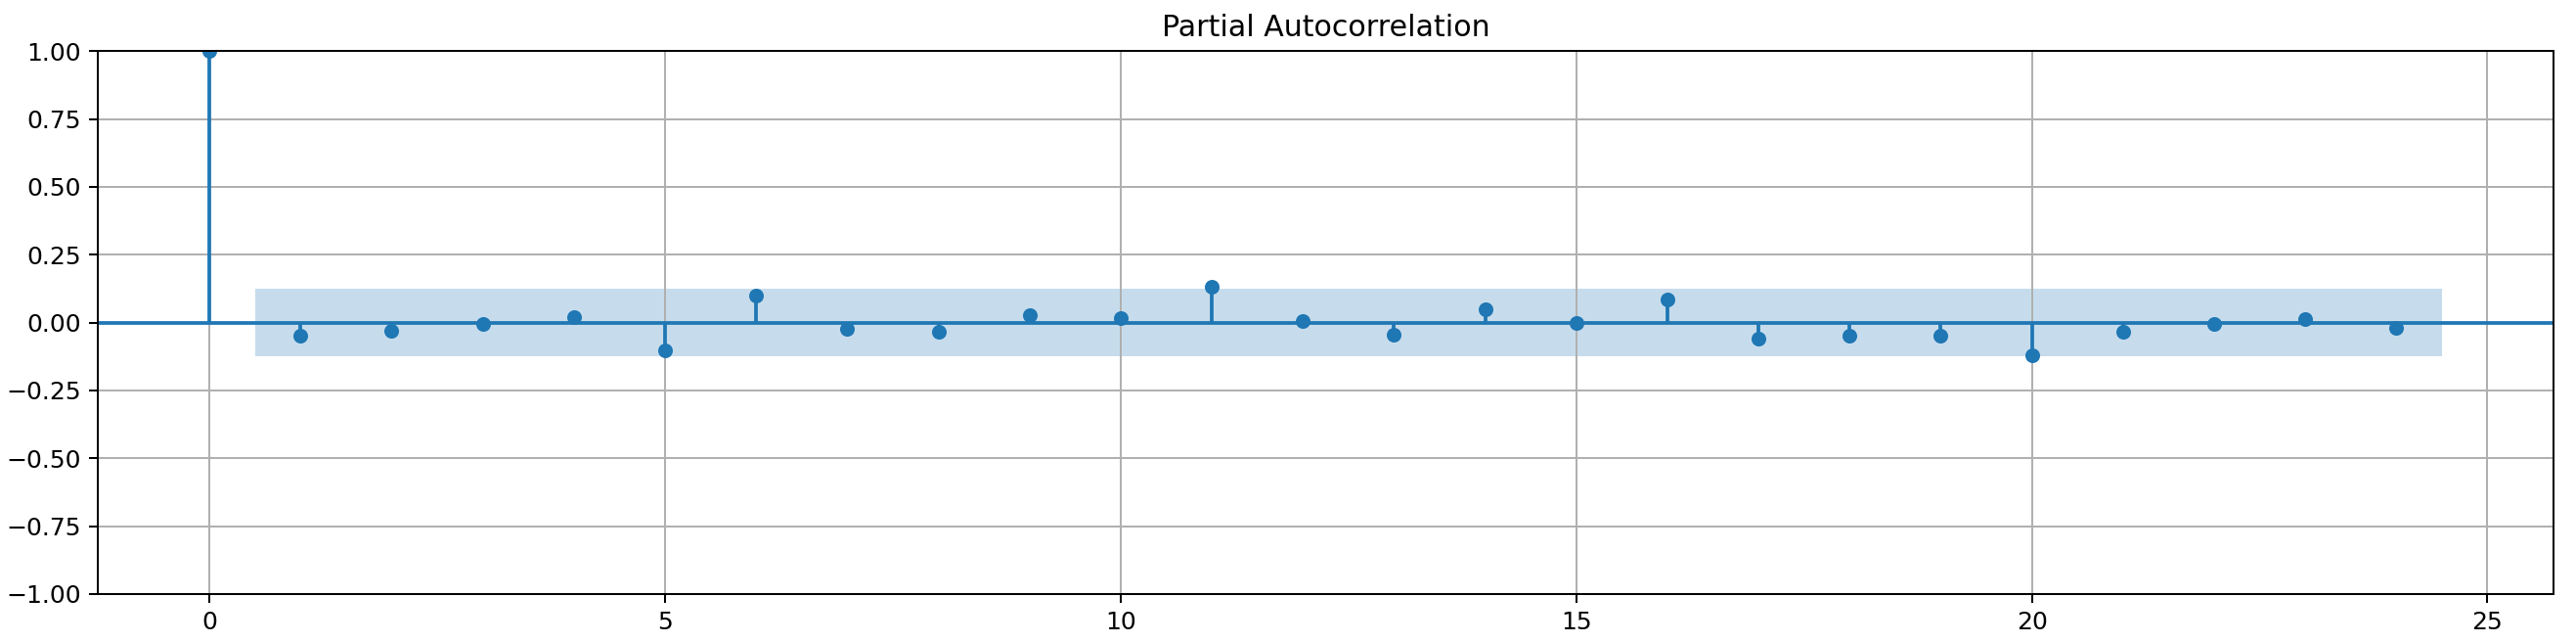
\includegraphics[width=17cm, height=5.1cm]{garch/garch_returns.png}
	\caption{PACF ряда доходностей (Apple цены открытия 2021)}
\end{figure}
\noindent Замечаем, что никаких значимых связей не наблюдается. Строим PACF для квадратов доходностей.
\begin{figure}[H]
	\centering
	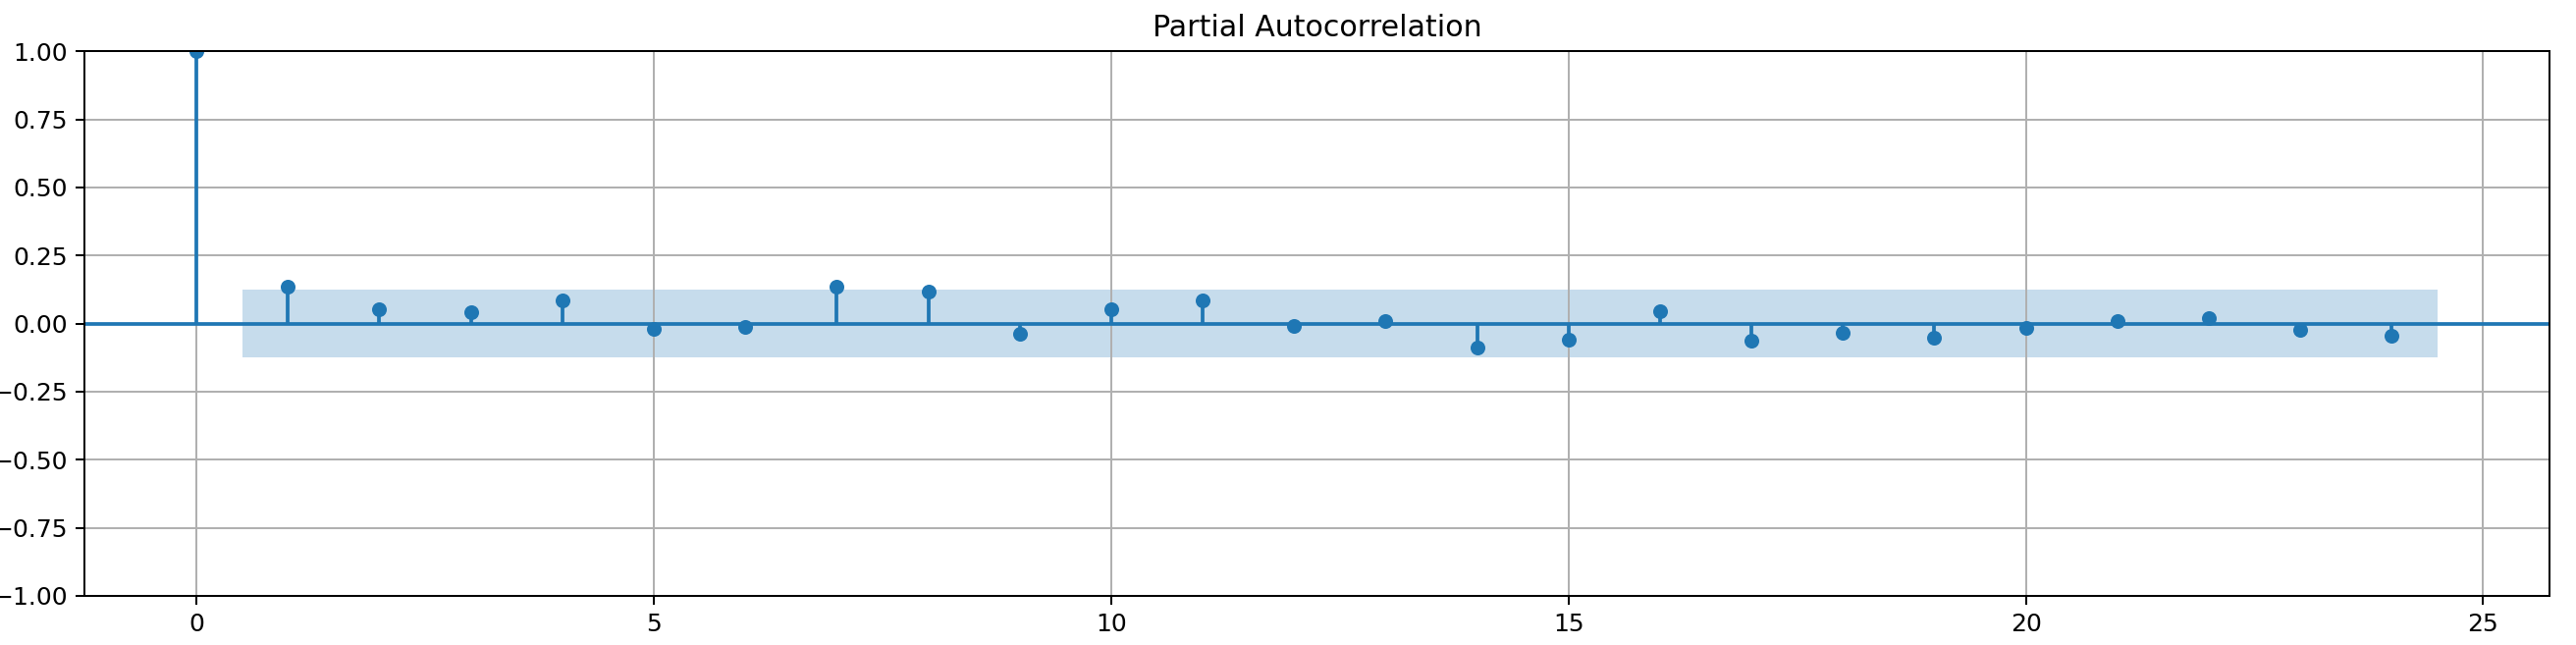
\includegraphics[width=17cm, height=5.1cm]{garch/garch_returns_sqr.png}
	\caption{PACF ряда квадратов доходностей (Apple цены открытия 2021)}
\end{figure}
\noindent Откуда получаем почти не значимый показатель для 1-ого лага, а этого уже достаточно, чтобы пытаться применить модель ARCH$(1)$. Несмотря на свою наглядность, только что показанный способ является необходимым, но не достаточным условием именно такого лага, значит, далее, основываясь на критерии BIC выбираем лучшую из обученных моделей модель. При этом моделирование среднего значения оставляем как классическое среднее, то есть: $\mu_t \equiv \mu$. Однако для большей уверенности в своих показателях, используем полноценный ряд доходностей компании Apple, начиная с ее выхода на IPO. Показатель доходности вычисляется на основе цен открытия.
\begin{figure}[H]
	\centering
	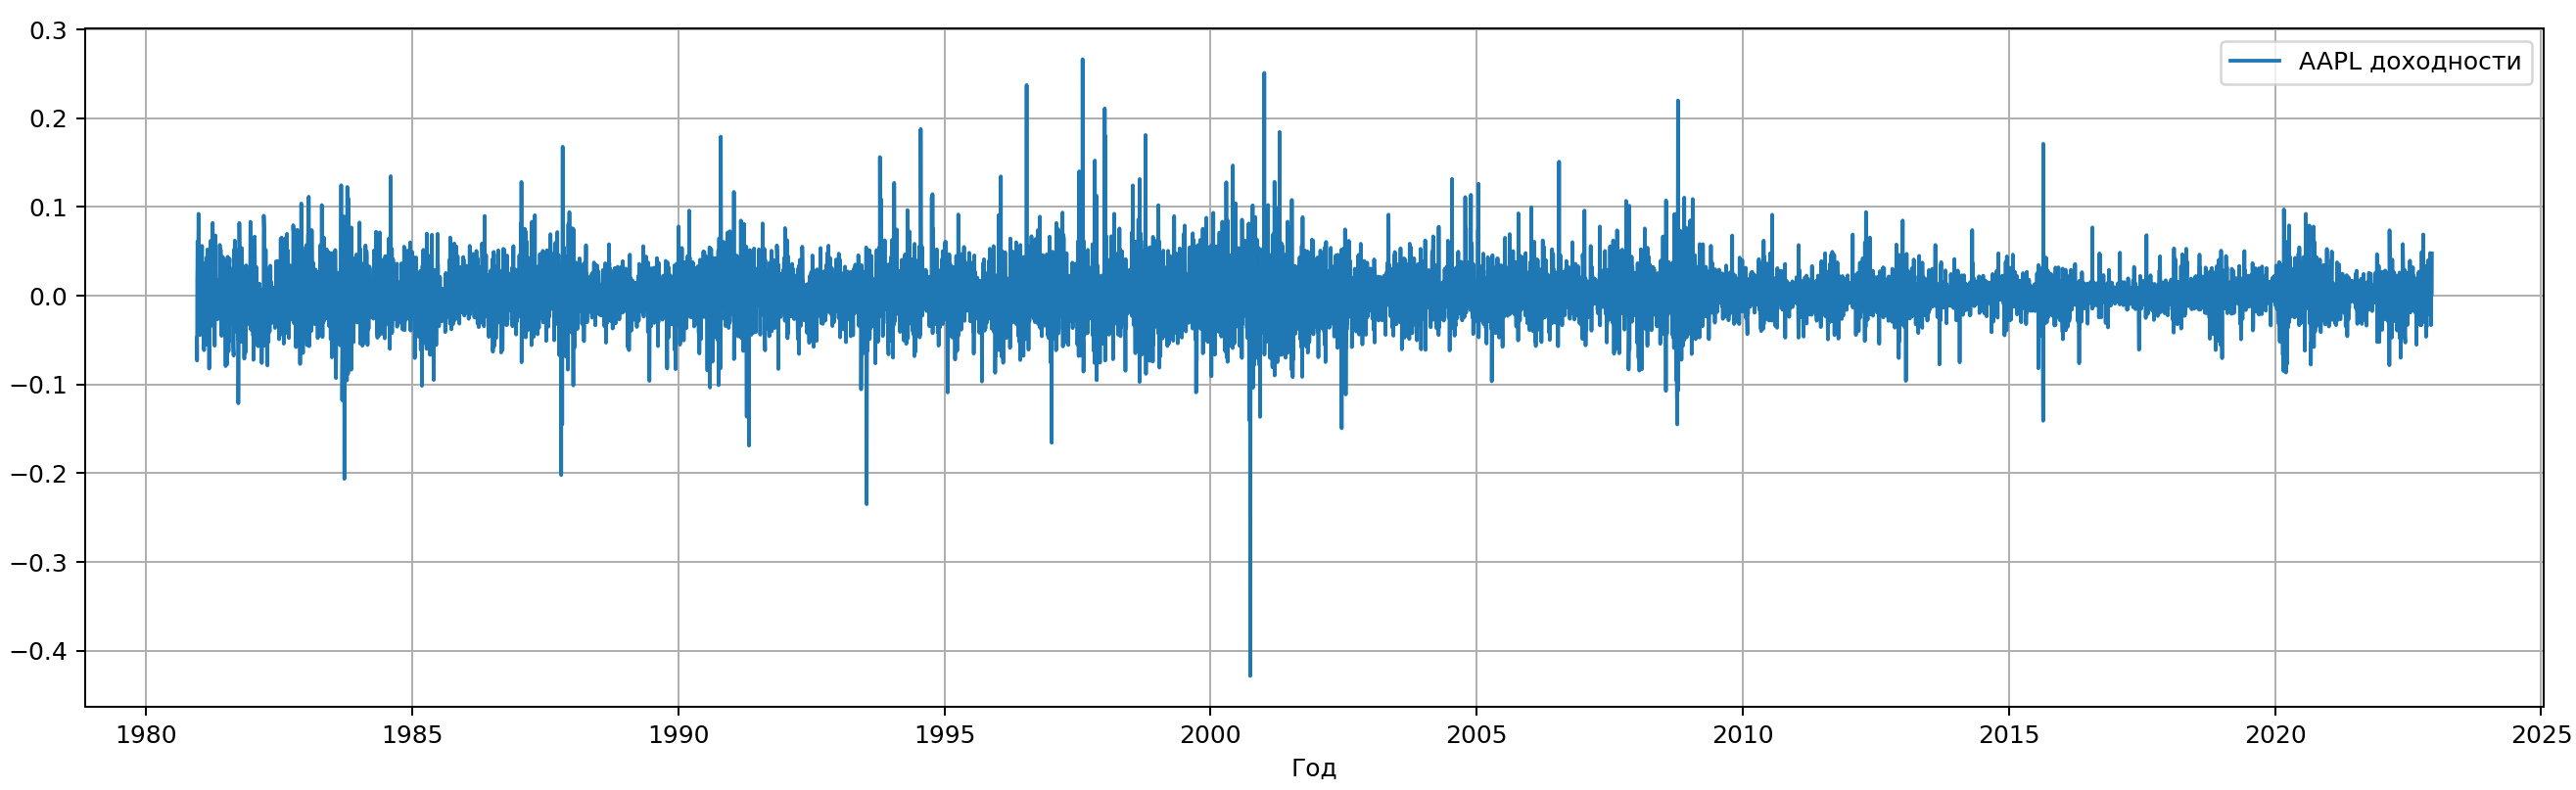
\includegraphics[width=17cm, height=4.5cm]{returns pictures/apple_returns.png}
	\caption{Доходности Apple (с выхода на IPO по 2022) не в \%}
\end{figure}
\noindent Квадраты доходностей соответственно имеют вид:
\begin{figure}[H]
	\centering
	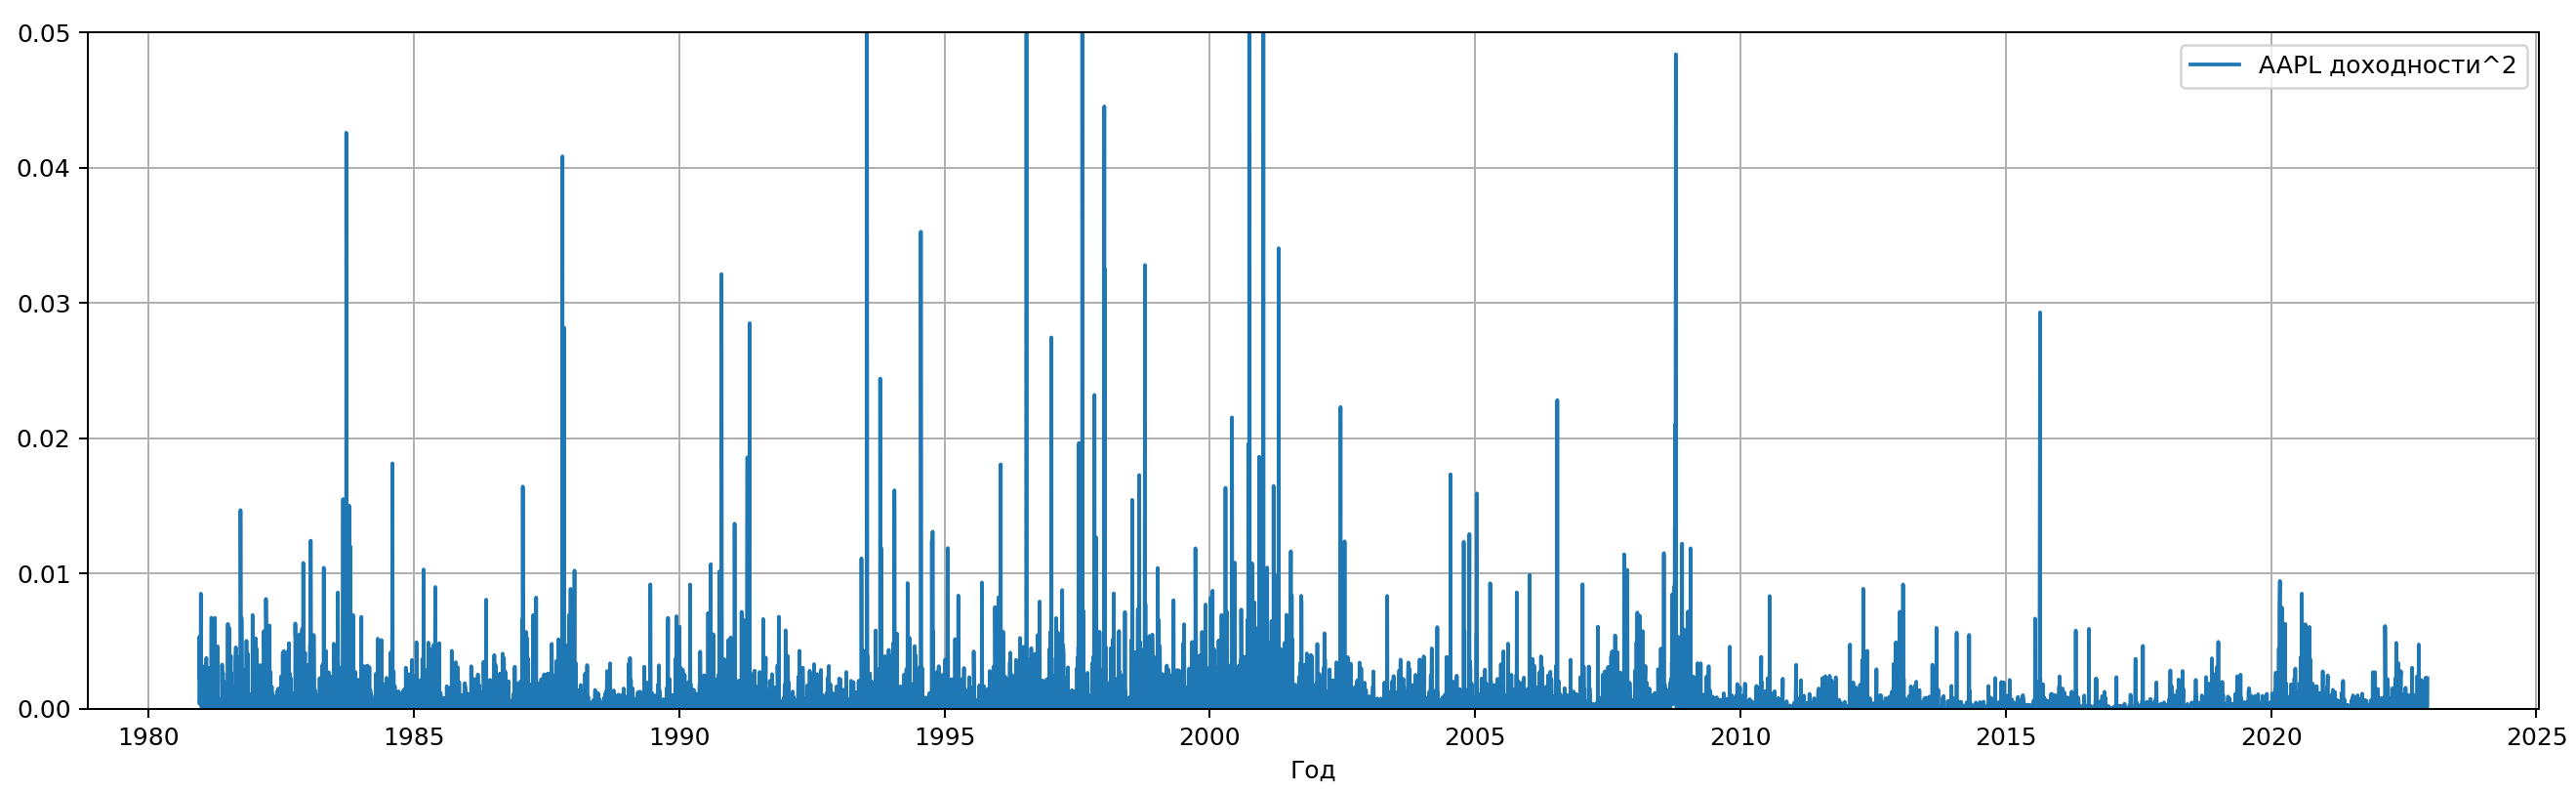
\includegraphics[width=17cm, height=4.5cm]{returns pictures/apple_returns_sqr.png}
	\caption{Квадраты доходностей Apple (с выхода на IPO по 2022) не в \%}
\end{figure}
\noindent Таким образом, им соответствующие PACF выглядят:
\begin{figure}[H]
	\centering
	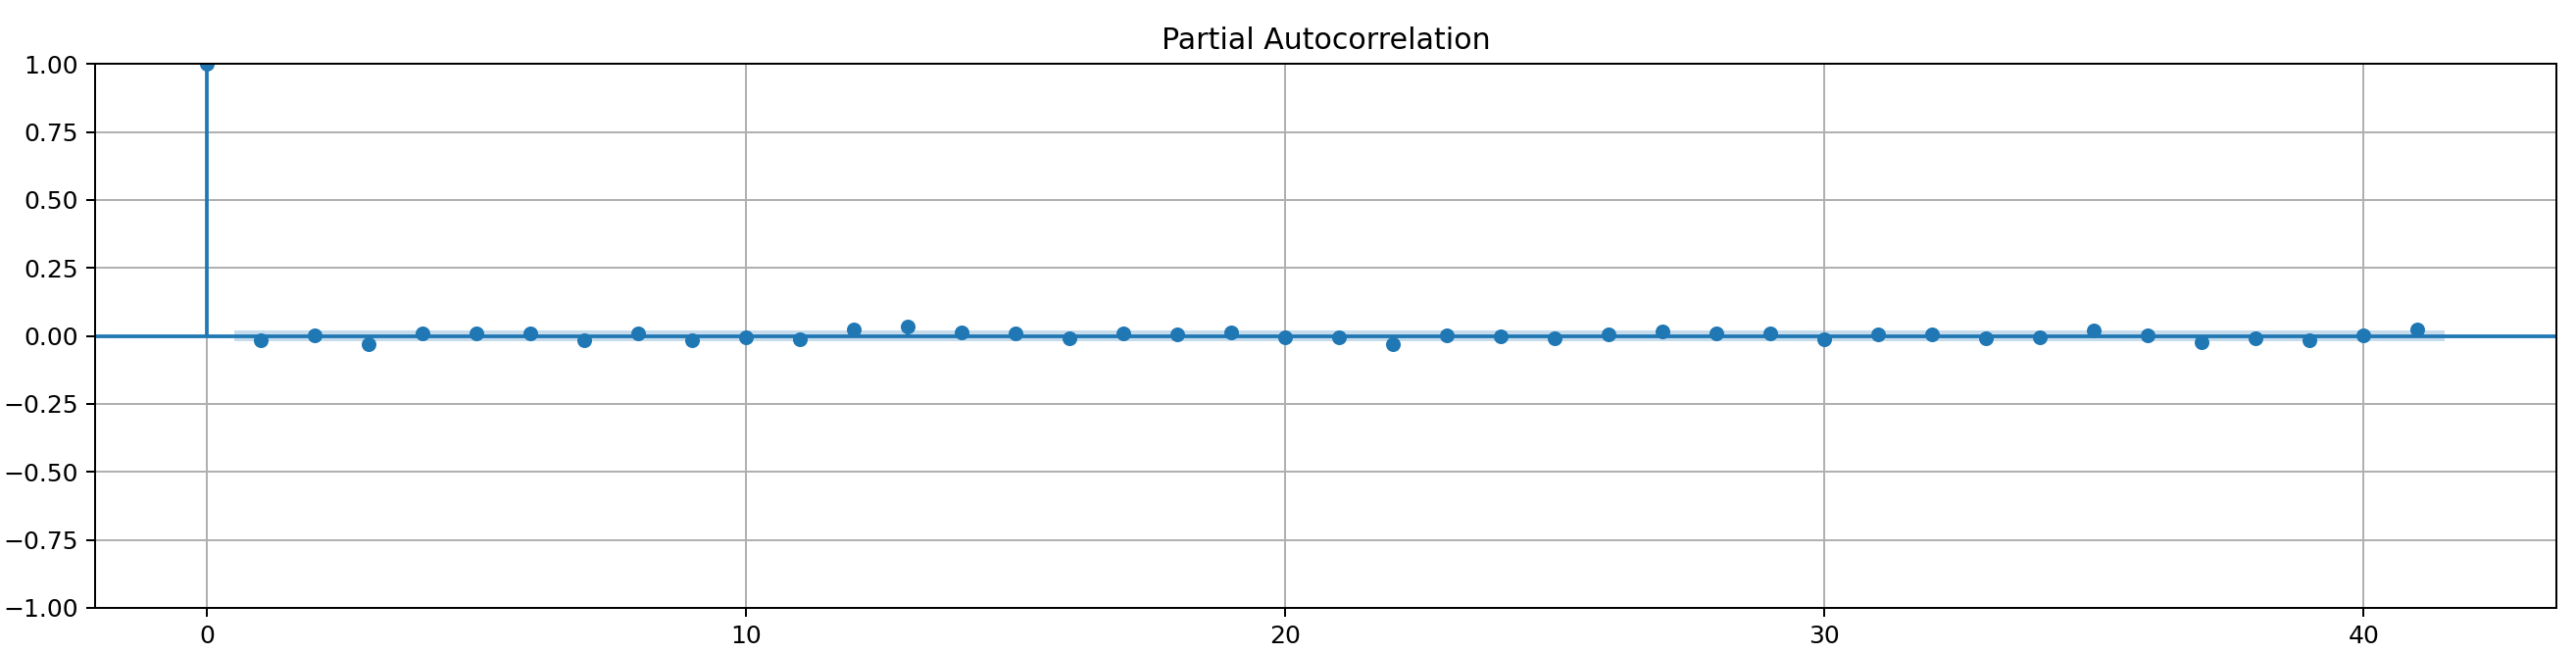
\includegraphics[width=17cm, height=4.5cm]{garch/garch_returns_long.png}
	\caption{PACF ряда доходностей Apple (с выхода на IPO по 2022)}
\end{figure}
\noindent Аналогично предыдущему случаю, никаких значимых связей тут тоже не наблюдается. Строим PACF для квадратов доходностей.
\begin{figure}[H]
	\centering
	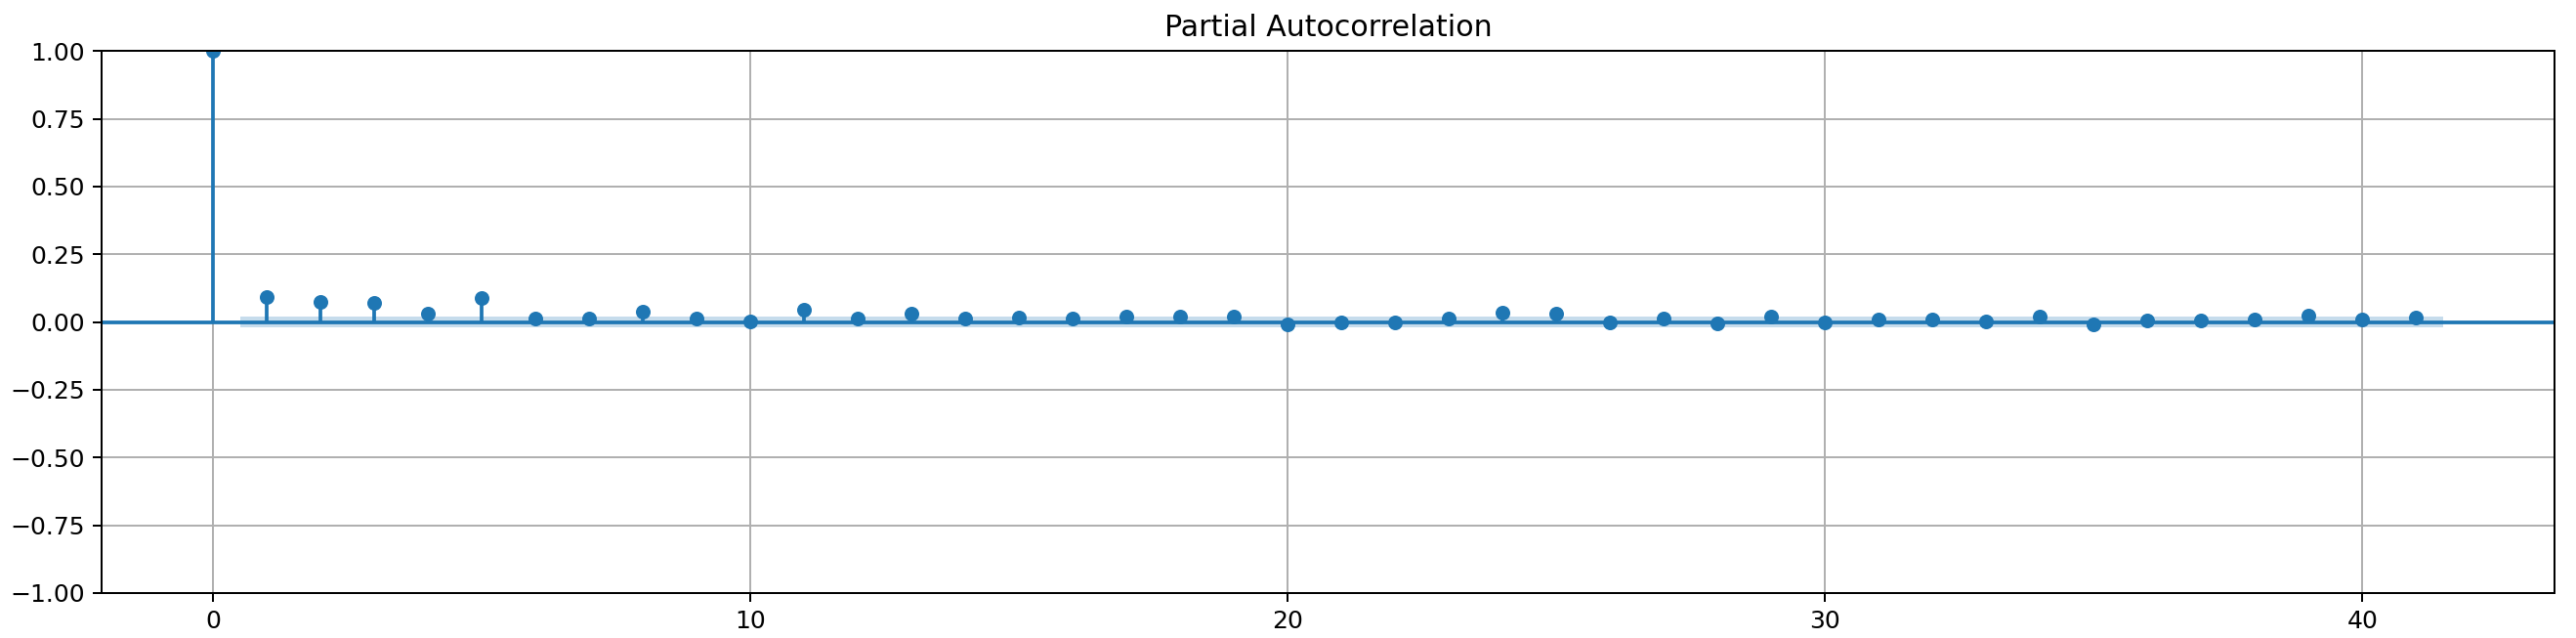
\includegraphics[width=17cm, height=4.5cm]{garch/garch_returns_sqr_long.png}
	\caption{PACF ряда квадратов доходностей Apple (с выхода на IPO по 2022)}
\end{figure}
\noindent А тут уже точно есть четко выраженная автокорреляционная зависимость, что однозначно сигнализирует о необходимости проверки моделей из ARCH семейства. Таким образом, для начала вычисляем GARCH$(p, q)$ такие, что $(p, q) \in \left\{(1, 1), (1, 2), (2, 1), (2, 2)\right\}$, а потом все ARCH$(p): p = \overline{1,10}$. Это делается для лучшего понимания, какая модель наиболее качественно описывает данные.

\begin{table}[H] \label{link::garchs}
	\centering
	\begin{tabular}{c|cccc}
		\toprule
		& GARCH$(1, 1)$ & GARCH$(1, 2)$ & GARCH$(2, 1)$ & GARCH$(2, 2)$\\
		\midrule[0.02cm]
		$\mu$ & \setval{0.174}{***}{0.024} & \setval{0.170}{***}{0.025} & \setval{0.174}{***}{0.028} & \setval{0.168}{}{0.159}\\[0.4cm]
		$\omega$ & \setval{0.073}{*}{0.024} & \setval{0.089}{**}{0.042} & \setval{0.073}{}{0.078} & \setval{0.119}{}{0.716}\\[0.4cm]
		$\alpha_1$ & \setval{0.068}{***}{0.024} & \setval{0.089}{***}{0.028} & \setval{0.068}{***}{0.014} & \setval{0.079}{}{0.228}\\[0.4cm]
		$\alpha_2$ & - & - & \setval{0.000}{}{0.051} & \setval{0.037}{}{0.053}\\[0.4cm]
		$\beta_1$ & \setval{0.927}{***}{0.026} & \setval{0.430}{}{0.772} & \setval{0.927}{***}{0.709} & \setval{0.000}{}{3.782}\\[0.4cm]
		$\beta_2$ & - & \setval{0.474}{}{0.757} & - & \setval{0.875}{}{3.243}\\
		\midrule[0.02cm]
		BIC & $50'056.5$ & $50'054.1$ & $50'065.7$ & $50'047.3$\\[0.05cm]
		$n$ & $10'590$ & $10'590$ & $10'590$ & $10'590$\\
		\midrule[0.02cm]
		Note: & \multicolumn{4}{r}{*$p < 0.1$, **$p < 0.05$, ***$p < 0.01$}\\
	\end{tabular}
	\caption{Сводная таблица моделей GARCH}
\end{table}



\begin{landscape}
	\begin{table}
	\centering
	\caption{Сводная таблица оцененных моделей. (*$p < 0.1$, **$p < 0.05$, ***$p < 0.01$)}
	\begin{tabular}{c|cccccccccc}
		\toprule
		& ARCH$(1)$ & ARCH$(2)$	& ARCH$(3)$	& ARCH$(4)$  & ARCH$(5)$  & ARCH$(6)$  & ARCH$(7)$ & ARCH$(8)$ & ARCH$(9)$ & ARCH$(10)$\\
		\midrule[0.02cm]
		$\mu$ & \setval{0.137}{***}{0.029} & \setval{0.175}{***}{0.029} & \setval{0.184}{***}{0.027} & \setval{0.178}{***}{0.026} & \setval{0.186}{***}{0.026} & \setval{0.187}{***}{0.026} & \setval{0.189}{***}{0.026} & \setval{0.188}{***}{0.025} & \setval{0.191}{***}{0.025} & \setval{0.191}{***}{0.025}\\[0.25cm]
		$\omega$ & \setval{5.993}{***}{0.241} & \setval{4.789}{***}{0.227} & \setval{3.891}{***}{0.205} & \setval{3.352}{***}{0.221} & \setval{3.002}{***}{0.195} & \setval{2.709}{***}{0.199} & \setval{2.408}{***}{0.198} & \setval{2.257}{***}{0.199} & \setval{2.135}{***}{0.202} & \setval{2.110}{***}{0.206}\\[0.25cm]
		$\alpha_1$ & \setval{0.307}{***}{0.054} & \setval{0.239}{***}{0.045} & \setval{0.227}{***}{0.048} & \setval{0.206}{***}{0.041} & \setval{0.174}{***}{0.028} & \setval{0.166}{***}{0.027} & \setval{0.149}{***}{0.024} & \setval{0.144}{***}{0.023} & \setval{0.140}{***}{0.022} & \setval{0.140}{***}{0.022}\\[0.25cm]
		$\alpha_2$ & - & \setval{0.0236}{***}{0.038} & \setval{0.218}{***}{0.036} & \setval{0.207}{***}{0.036} & \setval{0.169}{***}{0.034} & \setval{0.161}{***}{0.034} & \setval{0.150}{***}{0.034} & \setval{0.148}{***}{0.034} & \setval{0.142}{***}{0.031} & \setval{0.141}{***}{0.031}\\[0.25cm]
		$\alpha_3$ & - & - & \setval{0.163}{***}{0.026} & \setval{0.152}{***}{0.026} & \setval{0.144}{***}{0.025} & \setval{0.139}{***}{0.025} & \setval{0.125}{***}{0.024} & \setval{0.117}{***}{0.023} & \setval{0.116}{***}{0.023} & \setval{0.113}{***}{0.023}\\[0.25cm]
		$\alpha_4$ & - & - & - & \setval{0.122}{***}{0.028} & \setval{0.091}{***}{0.009} & \setval{0.083}{***}{0.019} & \setval{0.079}{***}{0.018} & \setval{0.069}{***}{0.017} & \setval{0.062}{***}{0.018} & \setval{0.059}{***}{0.018}\\[0.25cm]
		$\alpha_5$ & - & - & - & - & \setval{0.134}{***}{0.031} & \setval{0.112}{***}{0.030} & \setval{0.120}{***}{0.031} & \setval{0.111}{***}{0.029} & \setval{0.104}{***}{0.029} & \setval{0.104}{***}{0.029} \\[0.25cm]
		$\alpha_6$ & - & - & - & - & - & \setval{0.086}{***}{0.025} & \setval{0.084}{***}{0.026} & \setval{0.075}{***}{0.024} & \setval{0.067}{***}{0.022} & \setval{0.066}{***}{0.022}\\[0.25cm]
		$\alpha_7$ & - & - & - & - & - & - & \setval{0.093}{***}{0.026} & \setval{0.083}{***}{0.026} & \setval{0.080}{***}{0.026} & \setval{0.080}{***}{0.026}\\[0.25cm]
		$\alpha_8$ & - & - & - & - & - & - & - & \setval{0.067}{***}{0.019} & \setval{0.063}{***}{0.019} & \setval{0.063}{***}{0.019}\\[0.25cm]
		$\alpha_9$ & - & - & - & - & - & - & - & - & \setval{0.055}{**}{0.025} & \setval{0.052}{**}{0.025}\\[0.25cm]
		$\alpha_{10}$ & - & - & - & - & - & - & - & - & - & \setval{0.013}{}{0.013}\\
		\midrule[0.02cm]
		BIC & $51'448.5$ & $51'062.1$ & $50'785.2$ & $50'654.5$ & $50'427.6$ & $50'367.6$ & $50'301.6$ & $50'259.5$ & $50'240.5$ & $50'247.0$\\
		$n$ & $10'590$ & $10'590$ & $10'590$ & $10'590$ & $10'590$ & $10'590$ & $10'590$ & $10'590$ & $10'590$& $10'590$\\
		\midrule[0.02cm]
	\end{tabular}
\end{table}
\end{landscape}

